\documentclass{standalone}
\usepackage{tikz}
\usepackage{pgfplots}
\usepackage{xcolor}
\pgfplotsset{compat=1.14}

\usetikzlibrary{backgrounds}
\pgfdeclarelayer{foreground}
\pgfsetlayers{background,main,foreground}
\tikzset{%
	on foreground layer/.style={%
		execute at begin scope={%
			\pgfonlayer{foreground}%
			\let\tikz@options=\pgfutil@empty%
			\tikzset{every on foreground layer/.try,#1}%
			\tikz@options%
		},
		execute at end scope={\endpgfonlayer}
	},
	% addasu o ateb Loop Space: https://tex.stackexchange.com/a/20426/
	%\url{https://tex.stackexchange.com/q/46957/86}
	on layer/.code={%
		\pgfonlayer{#1}\begingroup
		\aftergroup\endpgfonlayer
		\aftergroup\endgroup
	},
	node on layer/.code={%
		\gdef\node@@on@layer{%
			\setbox\tikz@tempbox=\hbox\bgroup\pgfonlayer{#1}\unhbox\tikz@tempbox\endpgfonlayer\egroup}
		\aftergroup\node@on@layer
	},
}
\def\node@on@layer{\aftergroup\node@@on@layer}


\newlength\figurewidth
\newlength\figureheight

% Define all the colors
\definecolor{colorDyn}{RGB}{246, 255, 242}
\definecolor{colorDynBlock}{RGB}{200, 255, 174}
\definecolor{colorState}{RGB}{226, 255, 214}
\definecolor{colorStateBlock}{RGB}{154, 255, 100}
\definecolor{colorActivities}{RGB}{233, 255, 223}
\definecolor{colorActivitiesBlock}{RGB}{187, 255, 150}
\definecolor{colorActivitiesBlock2}{RGB}{171, 253, 128}
\definecolor{colorScen}{RGB}{255, 252, 204}
\definecolor{colorEgo}{RGB}{255, 204, 204}
\definecolor{colorStat}{RGB}{128, 128, 255}
\definecolor{colorLineStat}{RGB}{51, 51, 173}
\definecolor{colorLineDyn}{RGB}{51, 173, 51}

% Define main parts
\tikzstyle{block distance}=[node distance=6em]
\tikzstyle{block}=[draw, text width=5em, align=center, block distance, minimum height=2.8em, text depth=1.1em]
\tikzstyle{block one row}=[text depth=-0.1em]
\tikzstyle{dashed arrow}=[->, dashed, ultra thick]

% Define all kinds of distances
\tikzstyle{in between}=[coordinate, node distance=3em]
\tikzstyle{larger distance}=[node distance=6.5em]
\tikzstyle{environment text}=[coordinate, node distance=3.5em]
\tikzstyle{environment text b}=[node distance=0.2em, minimum width=6.5em, align=right]
\tikzstyle{entrance environment}=[coordinate, node distance=4.8em]
\tikzstyle{helper arrow}=[coordinate, node distance=2em]
\tikzstyle{top env box hwidth}=[coordinate, node distance=6.1em]
\tikzstyle{length dashed arrow}=[coordinate, node distance=2.5em]
\tikzstyle{distance heading}=[node distance=3em]
\tikzstyle{entrance states}=[coordinate, node distance=3.5em]
\tikzstyle{state below}=[coordinate, node distance=3em]
\tikzstyle{distance activities}=[node distance=7em]
\tikzstyle{entrance activities}=[coordinate, node distance=3.5em]
\tikzstyle{distance activities 2}=[node distance=5em]
\tikzstyle{margin dyn box}=[coordinate, node distance=0.3em]
\tikzstyle{activities below}=[coordinate, node distance=2em]

\begin{document}

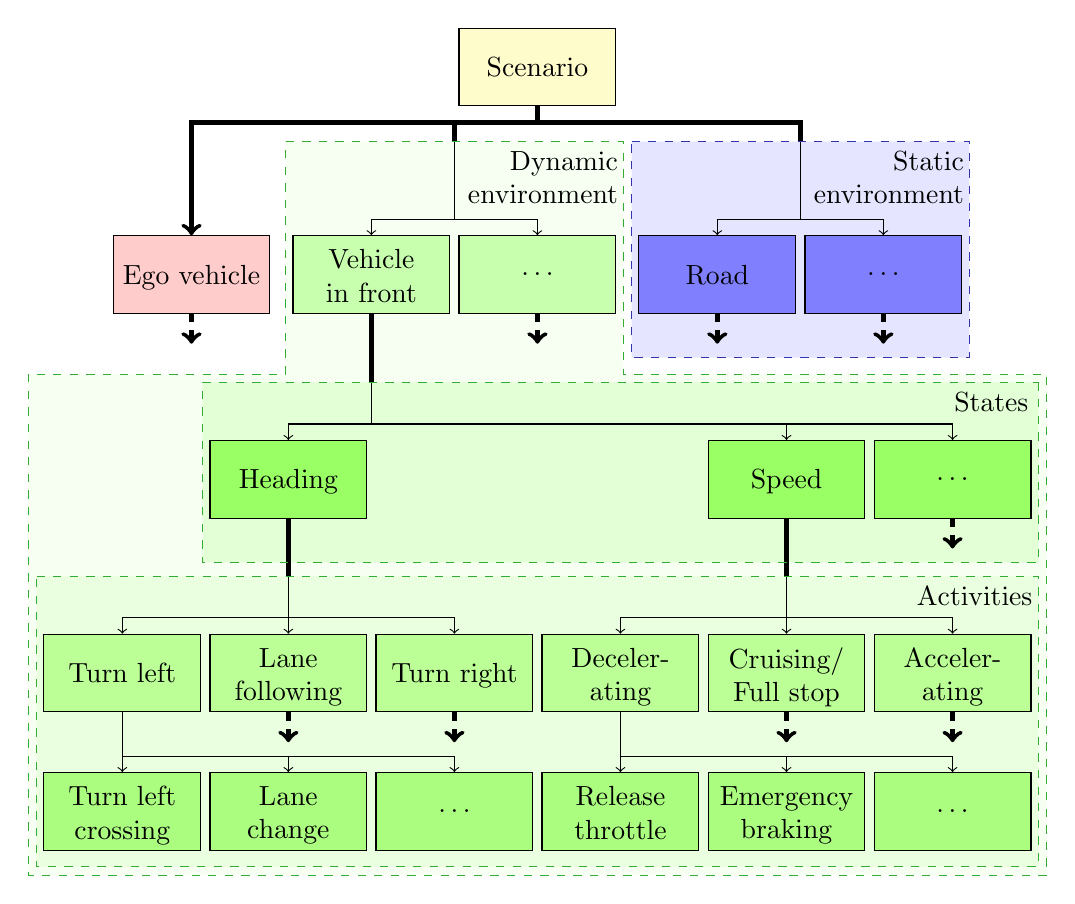
\begin{tikzpicture}
	\node[block, fill=colorScen, block one row](scenario){Scenario};
	\node[coordinate, below of=scenario, node distance=2em](helper scenario){};
	
	% Create dynamic environment
	\node[coordinate, below of=scenario, node distance=7.5em](below scenario){};
	\node[fill=colorDynBlock, block, left of=below scenario, node distance=0em, block one row](otherdyn){$\ldots$};
	\node[length dashed arrow, below of=otherdyn](otherdyn arrow){};
	\draw[dashed arrow] (otherdyn) -- (otherdyn arrow);
	\node[fill=colorDynBlock, block, left of=otherdyn](target){Vehicle in front};
	\node[above of=otherdyn, environment text](helper1){};
	\node[right of=helper1, environment text b]{Dynamic\\environment};
	\node[left of=otherdyn, in between](helper2){};
	\node[entrance environment, above of=helper2](entrance dyn){};
	\node[helper arrow, above of=helper2](helper dyn){};
	\draw[ultra thick] (scenario) -- (helper scenario) -| (entrance dyn);
	\draw[->] (entrance dyn) -- (helper dyn) -| (target);
	\draw[->] (entrance dyn) -- (helper dyn) -| (otherdyn);
	
	% Ego vehicle
	\node[block, larger distance, left of=target, fill=colorEgo, block one row](ego){Ego vehicle};
	\draw[ultra thick, ->] (scenario) --(helper scenario) -| (ego);
	\node[length dashed arrow, below of=ego](ego arrow){};
	\draw[dashed arrow] (ego) -- (ego arrow);
	
	% Static environment
	\node[block, right of=otherdyn, larger distance, fill=colorStat, block one row](road){Road};
	\node[block, right of=road, fill=colorStat, block one row](weather){$\ldots$};
	\node[above of=weather, environment text](helper3){};
	\node[right of=helper3, environment text b]{Static\\environment};
	\node[left of=weather, in between](helper4){};
	\node[entrance environment, above of=helper4](entrance stat){};
	\node[helper arrow, above of=helper4](helper stat){};
	\draw[ultra thick] (scenario) -- (helper scenario) -| (entrance stat);
	\draw[->] (entrance stat) -- (helper stat) - | (road);
	\draw[->] (entrance stat) -- (helper stat) - | (weather);
	\node[length dashed arrow, below of=road](road arrow){};
	\draw[dashed arrow] (road) -- (road arrow);
	\node[length dashed arrow, below of=weather](weather arrow){};
	\draw[dashed arrow] (weather) -- (weather arrow);
	
	% States
	\node[coordinate, below of=target, node distance=7.4em](below target){};
	\node[fill=colorStateBlock, block, left of=below target, distance heading, block one row](heading){Heading};
	\node[fill=colorStateBlock, block, right of=below target, node distance=15em, block one row](speed){Speed};
	\node[fill=colorStateBlock, block, right of=speed, block one row](other states){$\ldots$};
	\node[coordinate, above of=other states, node distance=2.8em](helper10){};
	\node[right of=helper10, node distance=1.4em, minimum width=4em, align=right]{States};
	\node[above of=heading, entrance states](helper17){};
	\node[coordinate, right of=helper17, distance heading](entrance states){};
	\node[coordinate, below of=target, node distance=5.4em](helper states){};
	\draw[ultra thick] (target) -- (entrance states);
	\draw[->] (entrance states) -- (helper states) -| (heading);
	\draw[->] (entrance states) -- (helper states) -| (speed);
	\draw[->] (entrance states) -- (helper states) -| (other states);
	\node[length dashed arrow, below of=other states](other states arrow){};
	\draw[dashed arrow] (other states) -- (other states arrow);
	
	% Activities for heading
	\node[fill=colorActivitiesBlock, block, below of=heading, distance activities](lane following){Lane following};
	\node[fill=colorActivitiesBlock, block, left of=lane following, block one row](left){Turn left};
	\node[fill=colorActivitiesBlock, block, right of=lane following, block one row](right){Turn right};
	\node[entrance activities, above of=lane following](entrance heading){};
	\node[helper arrow, above of=lane following](helper heading){};
	\draw[ultra thick] (heading) -- (entrance heading);
	\draw[->] (entrance heading) -- (helper heading) -| (left);
	\draw[->] (entrance heading) -- (lane following);
	\draw[->] (entrance heading) -- (helper heading) -| (right);
	\node[length dashed arrow, below of=lane following](lane following arrow){};
	\node[length dashed arrow, below of=right](right arrow){};
	\draw[dashed arrow] (lane following) -- (lane following arrow);
	\draw[dashed arrow] (right) -- (right arrow);
	
	% Activities for speed
	\node[fill=colorActivitiesBlock, block, below of=speed, distance activities](cruising){Cruising/ Full stop};
	\node[fill=colorActivitiesBlock, block, left of=cruising](decelerating){Deceler-ating};
	\node[fill=colorActivitiesBlock, block, right of=cruising](accelerating){Acceler-ating};
	\node[entrance activities, above of=cruising](entrance speed){};
	\node[helper arrow, above of=cruising](helper speed){};
	\draw[ultra thick] (speed) -- (entrance speed);
	\draw[->] (entrance speed) -- (helper speed) -| (decelerating);
	\draw[->] (entrance speed) -- (cruising);
	\draw[->] (entrance speed) -- (helper speed) -| (accelerating);
	\node[length dashed arrow, below of=cruising](cruising arrow){};
	\node[length dashed arrow, below of=accelerating](accelerating arrow){};
	\draw[dashed arrow] (cruising) -- (cruising arrow);
	\draw[dashed arrow] (accelerating) -- (accelerating arrow);
	
	% Possibilities for turning left
	\node[fill=colorActivitiesBlock2, block, below of=left, distance activities 2](crossing){Turn left crossing};
	\node[fill=colorActivitiesBlock2, block, right of=crossing](lane change){Lane change};
	\node[fill=colorActivitiesBlock2, block, right of=lane change, block one row](other left){$\ldots$};
	\node[helper arrow, above of=crossing](helper left){};
	\draw[->] (left) -- (crossing);
	\draw[->] (left) -- (helper left) -| (lane change);
	\draw[->] (left) -- (helper left) -| (other left);
	
	% Possibilities for decelerating
	\node[fill=colorActivitiesBlock2, block, below of=decelerating, distance activities 2](release){Release throttle};
	\node[fill=colorActivitiesBlock2, block, right of=release](emergency){Emergency braking};
	\node[fill=colorActivitiesBlock2, block, right of=emergency, block one row](other decelerating){$\ldots$};
	\node[helper arrow, above of=release](helper decelerating){};
	\draw[->] (decelerating) -- (release);
	\draw[->] (decelerating) -- (helper decelerating) -| (emergency);
	\draw[->] (decelerating) -- (helper decelerating) -| (other decelerating);
	
	% Define all the nodes for the dashed boxes %%%%%%%%%%%%%%%%%%%%%%%%%%%%%%%%%%%%%%%%%%%%%
	% Dashed box around static environment
	\node[top env box hwidth, left of=entrance stat](helper5){};
	\node[top env box hwidth, right of=entrance stat](helper6){};
	\node[coordinate, below of=helper4, node distance=3em](helper7){};
	\node[top env box hwidth, left of=helper7](helper8){};
	\node[top env box hwidth, right of=helper7](helper9){};
	
	% Dashed box around states (this is done in a strange manner, but this way
	% we make sure the margins are similar as for the environment blocks)
	\node[below of=other states, state below](helper13){};
	\node[left of=helper13, in between](helper11){};
	\node[right of=helper11, top env box hwidth](helper12){};
	\node[below of=heading, state below](helper16){};
	\node[right of=helper16, in between](helper14){};
	\node[left of=helper14, top env box hwidth, red](helper15){};
	\node[right of=helper17, in between](helper18){};
	\node[left of=helper18, top env box hwidth](helper19){};
	\node[above of=other states, entrance states](helper20){};
	\node[left of=helper20, in between](helper21){};
	\node[right of=helper21, top env box hwidth](helper22){};
	
	% Box around activities and label for activities
	\node[entrance activities, above of=left](helper23){};
	\node[right of=helper23, in between](helper24){};
	\node[left of=helper24, top env box hwidth](helper25){};
	\node[entrance activities, above of=accelerating](helper26){};
	\node[left of=helper26, in between](helper27){};
	\node[right of=helper27, top env box hwidth](helper28){};
	\node[below of=other decelerating, activities below](helper29){};
	\node[left of=helper29, in between](helper30){};
	\node[right of=helper30, top env box hwidth](helper31){};
	\node[below of=crossing, activities below](helper32){};
	\node[right of=helper32, in between](helper33){};
	\node[left of=helper33, top env box hwidth](helper34){};
	\node[coordinate, above of=accelerating, node distance=2.8em](helper35){};
	\node[right of=helper35, node distance=0.8em, minimum width=4em, align=right]{Activities};
	
	% Box for dynamic environment
	\node[top env box hwidth, left of=entrance dyn](helper36){};
	\node[top env box hwidth, right of=entrance dyn](helper37){};
	\node[margin dyn box, above of=entrance states](helper38){};
	\node[right of=helper38, in between](helper39){};
	\node[left of=helper39, top env box hwidth](helper40){};
	\node[right of=helper39, top env box hwidth](helper41){};
	\node[right of=helper31, margin dyn box](helper42){};
	\node[below of=helper42, margin dyn box](helper43){};
	\node[left of=helper34, margin dyn box](helper44){};
	\node[below of=helper44, margin dyn box](helper45){};
	
	% Draw the boxes
	% Static environment
	\draw[dashed, color=colorLineStat] (helper5) -- (helper6) -- (helper9) -- (helper8) -- (helper5);
	\fill[fill=blue!10, on layer=background] (helper5) -- (helper6) -- (helper9) -- (helper8) -- (helper5);
	
	% Dynamic environment
	\draw[dashed, color=colorLineDyn] (helper36) -- (helper37) -- (helper41) -| (helper43) -- (helper45) |- (helper40) -- (helper36);
	\fill[fill=colorDyn, on layer=background] (helper36) -- (helper37) -- (helper41) -| (helper43) -- (helper45) |- (helper40) -- (helper36);
	
	% States
	\draw[dashed, color=colorLineDyn] (helper22) -- (helper12) -- (helper15) -- (helper19) -- (helper22);
	\fill[fill=colorState, on layer=background] (helper22) |- (helper12) -- (helper15) -- (helper19) -- (helper22);
	
	% Activities
	\draw[dashed, color=colorLineDyn] (helper25) -- (helper28) -- (helper31) -- (helper34) -- (helper25);
	\fill[fill=colorActivities, on layer=background] (helper25) |- (helper28) -- (helper31) -- (helper34) -- (helper25);
\end{tikzpicture}
	
\end{document}
